\documentclass{article}
\RequirePackage[a4paper,top=1.8cm,bottom=2.54cm,outer=1.0cm,textwidth=7in,twoside,includefoot,includehead,nofoot]{geometry}
\usepackage{graphicx}
\def\Eo{\mbox{\sc Ezo}}
\def\Ec{\mbox{\sc Ezo-CNN}}
\def\Hite{\mbox{\sc Hexcited}}
\def\Hent{\mbox{\sc Hexcellent}}
\def\Mx{\mbox{\sc MoHex}}
\def\Mc{\mbox{\sc MoHex-CNN}}
\def\Sol{\mbox{\sc Solver}}
\def\Fuego{\mbox{\sc Fuego}}

\begin{document}
\begin{figure}[hbt]
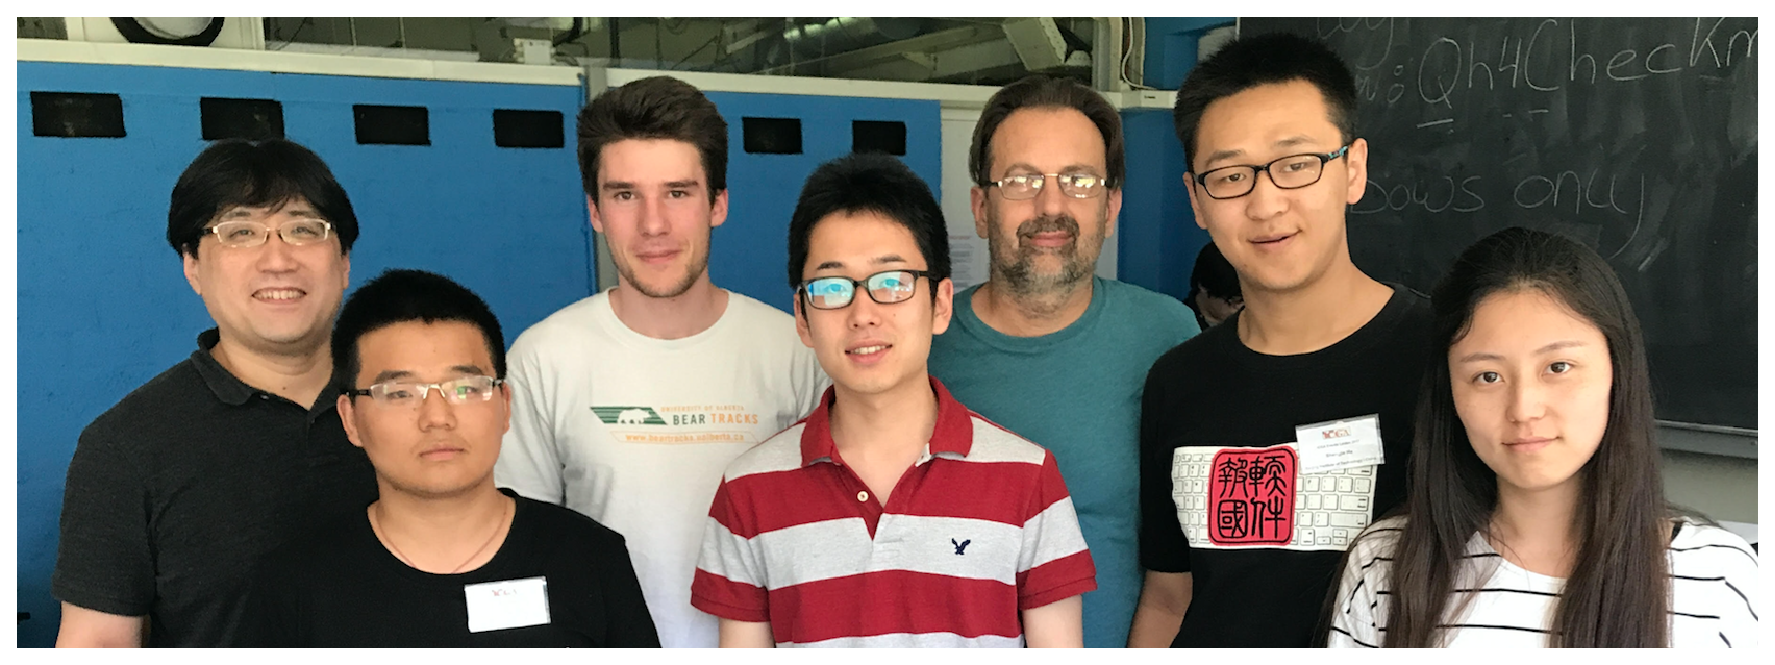
\includegraphics[width=\columnwidth]{photos/people-1.eps}\
\caption{Participants at the Hex competitions. From left,
Masahito Yamamoto,
You RunZe,
Noah Weninger,
Kei Takada,
Ryan Hayward,
Ma Shengjie,
Wu Tong.} \end{figure}


\begin{figure}[htp]
\noindent\hspace*{-1cm}\
\includegraphics[scale=.9]{pix/11.mh1.eps}\hspace*{-1cm}
\includegraphics[scale=.9]{pix/11.hm2.eps}\hspace*{-1cm}\
\includegraphics[scale=.9]{pix/11.mh3.eps}\hspace*{-1cm}\
\includegraphics[scale=.9]{pix/11.hm4.eps}
\caption{\Hite-\Mx\ Games 1-4. M-H 1-0, H-M 0-1, M-H 1-0, H-M 0-1.}
\end{figure}


\begin{figure}[hbp]
\noindent\
\includegraphics[scale=1]{pix/11.eh1.eps}\hspace*{-1cm}\
\includegraphics[scale=1]{pix/11.he2.eps}\hspace*{-1cm}\
\includegraphics[scale=1]{pix/11.eh3.eps}
\caption{\Hite-\Ec\ Games 1-3. E-H 1-0, H-E 0-1, E-H 1-0.
In Game 1, Black finishes with one of {\bf \{e8,h7\}}.}
\end{figure}

\begin{figure}[hbp]
\noindent\
\includegraphics[scale=1]{pix/11.em1plus.eps}\hspace*{-1cm}\
\includegraphics[scale=1]{pix/11.me2plus.eps}\hspace*{-1cm}\
\includegraphics[scale=1]{pix/11.em3plus.eps}

~

\noindent\
\includegraphics[scale=1]{pix/11.me4plus.eps}\hspace*{-1cm}\
\includegraphics[scale=1]{pix/11.me5plus.eps}\hspace*{-1cm}\
\includegraphics[scale=1]{pix/11.em6plus.eps}

~

\noindent\
\includegraphics[scale=1]{pix/11.me7plus.eps}\hspace*{-1cm}\
\includegraphics[scale=1]{pix/11.em8plus.eps}\hspace*{-1cm}\
\includegraphics[scale=1]{pix/11.em9plus.eps}
\caption{\Ec-\Mx\ Games.
a) 1-3. E-M 0-1, M-E 1-0, E-M 1-0.
b) 4-6. M-E 1-0, M-E 0-1, E-M 1-0.
c) 7-9. M-E 0-1, E-M 0-1, E-M 0-1.}
\label{fig:EM11}
\end{figure}

\newpage
\begin{figure}[hbp]
\noindent
\includegraphics[scale=1]{pix/11.me10plus.eps}\hspace*{-1cm}\
\includegraphics[scale=1]{pix/11.me11plus.eps}\hspace*{-1cm}\
\includegraphics[scale=1]{pix/11.em12plus.eps}
\caption{\Ec-\Mx\ Games 10-12. M-E 0-1, M-E 1-0, E-M 0-1.}
\end{figure}

\begin{figure}[hbp]
\noindent\hspace*{-.4cm}\
\includegraphics[scale=.9]{pix/13.hm1.eps}\hspace*{-1cm}\
\includegraphics[scale=.9]{pix/13.mh2.eps}\hspace*{-1cm}\
\includegraphics[scale=.9]{pix/13.eh1.eps}

~

\noindent\hspace*{-.4cm}\
\includegraphics[scale=.9]{pix/13.he2.eps}\hspace*{-1cm}\
\includegraphics[scale=.9]{pix/13.eh3.eps}\hspace*{-1cm}\
\includegraphics[scale=.9]{pix/13.he4.eps}
\caption{\Hent{} Games.  a) 1-3. H-M 0-1, M-H 1-0, E-H 1-0.
b) 4-6. H-E 0-1, E-H 1-0, H-E 0-1.}
\end{figure}

\begin{figure}[hbp]
\noindent\hspace*{-.4cm}\
\includegraphics[scale=.9]{pix/13.me1plus.eps}\hspace*{-1cm}\
\includegraphics[scale=.9]{pix/13.em2plus.eps}\hspace*{-1cm}\
\includegraphics[scale=.9]{pix/13.me3plus.eps}

~

\noindent\hspace*{-.4cm}\
\includegraphics[scale=.9]{pix/13.em4plus.eps}\hspace*{-1cm}\
\includegraphics[scale=.9]{pix/13.me5plus.eps}\hspace*{-1cm}\
\includegraphics[scale=.9]{pix/13.em6plus.eps}\

~

\noindent\hspace*{-.4cm}\
\includegraphics[scale=.9]{pix/13.me7plus.eps}\hspace*{-1cm}\
\includegraphics[scale=.9]{pix/13.em8plus.eps}
\caption{\Ec{}-\Mc\ Games. 
a) 1-3. M-E 1-0, E-M 1-0, M-E 0-1.
b) 4-6. E-M 0-1, M-E 1-0, E-M 0-1.
c) 7-8. M-E 1-0, E-M 0-1.}
\label{fig:EM13}
\end{figure}
\end{document}
